% -*- TeX-master:"main" -*-

\chapter{Automation Objects}
\label{automationobjects}
%% Intro
With the function blocks the main technological problem of
distributed automation has been solved. A general framework
for development and deployment of distributed automation
systems has been established. What is still needed is a way
of encapsulating function blocks together with the data
about their properties and, more importantly, about their
functionality in a way that will enable diminishing of the
time-to-market and facilitate effective rapid object
oriented development of automation systems. In this chapter
the concept of automation objects is presented as far as the
research has come. There are still plenty of details to be
worked out but this chapter should clarify the role and the
benefits of using the automation objects in the development
of the industrial, as well as other, automated control
systems.


\section{Background}
%% Background. Why automation objects? What do we want to do?
Considering the following arguments it is clear why such
encapsulation is needed and how it can help in achieving the
afore mentioned goal.

%%     effective reuse of software
Object oriented system development as presented in the
IEC~61499 standard is ideal for the purpose that it is
designed for but not enough for achieving effective software
reuse in automation systems development.

%%     effective decentralization of software development 
Effective software reuse facilitates effective
decentralization of software development. If anyone could
use the software that somebody else developed without
wasting time on resolving the difficulties that arise from
poorly documented interfaces, or resorting to
reimplementation because of the same problem, than everyone
could concentrate on providing the best implementation for
their part of the automation system software.

%%     easier integration and deployment of software
Leveraging effective software reuse and decentralized
software development makes integration and deployment much
easier. System integrator's task is hereby reduced to
picking the right software objects from the library and
connecting them for the specific application.

%%     development of libraries
Using the encapsulation of software objects with well
specified information about their usage makes it possible to
build libraries of elements that can easily be shared over
the Internet since everything that is needed for the usage
of the elements comes with the elements themselves. This is
unlike the Java system where the objects are distributed in
binary only format and the interface documentation has to be
downloaded or reviewed on-line prior to usage.

%%     all of these result in rapid development of
%%     automation systems
The arguments presented are enough to support the idea that
the software objects encapsulated with the information about
their usage will increase the speed of the development of
the automation systems.



\section{Specification}
To realize all of the above mentioned arguments a new kind
of software objects are needed, preliminary called
\emph{automation objects}. Even though this kind of objects
are still very much a research subject the following is the
specification of the objects so far.

%* AO consists of models, controllers, views and
%  configuration registry
Automation objects consists of models, controllers, views
and configuration registry implemented using IEC~61499
function blocks and their interfaces, see
figure~\ref{fig:AO}. Models are interchangeable simulation
models with varying level of abstraction. One model might
be used for the simulation on a high level of abstraction,
typically behavioral model, and another for the simulation
on a lower level. This is then used to implement dynamic
zooming during the simulation. One of the models will
implement the communication with the controlled equipment
thus allowing effortless switching between simulation and
actual control. This will enable gradual verification and
on-line tuning of the big automation systems by allowing the
simulation of the system components that are being
configured or tuned while running the components that are
already configured.
\begin{figure}[!ht]
  \centering
  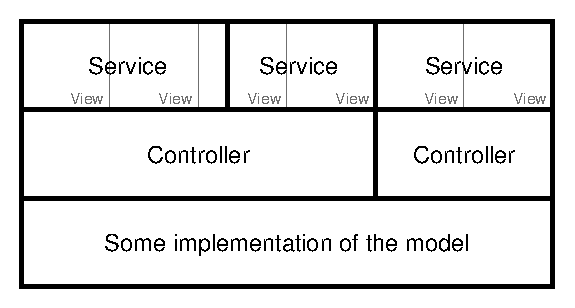
\includegraphics{images/automationobjects/AO}
  \caption{The architecture of the automation object.}
  \label{fig:AO}
\end{figure}

Controllers are function blocks that control the model. The
best examples of controllers are regulators as PI- or
PID-regulator. On the higher level of the automation system
these can be configurable implementations of different
automation algorithms. This allows interchange of different
controlling strategies for easy verification with simulation
and the equipment. The automation object can have as many
controllers as it is needed but only one controller may be
active at any time.

Views are the function blocks allowing user interaction with
the automation object. These implement all the allowable ways
of interaction with the automation object. At the lower
levels of the automation system they will typically provide
various interfaces to the object depending on the user's
needs while at the higher levels they will implement the
full graphical user interfaces for the operators. As with
the controllers there may be as many views as needed for the
automation object.

Configuration registry is a function block implementing the
configuration database and interface to it. This function
block holds all relevant attributes and configuration
variables for the automation object and provides an
interface for accessing and changing them. Configuration
registry is used by models, controllers and the views for
storing and retrieving the configuration data. For example,
controllers will use this function block to access their
regulator parameters and other configurable parameters.

%* Service is a set of views that support some relevant task
%  for the connected controller  
For every automation object a number of services may be
defined. A number of views that are needed for a certain
task during the development of the control system are
specified in the definition of the service thus the service
operates on a certain controller. The service can than be
invoked during the development and ease the task that it is
designed for. One service may only include views that
operate on the same controller since only one controller is
active at any time. Several services that operate on the
same controller may be activated at the same time. On the
other hand, services that operate on different controllers
are mutually exclusive. During the development of the
control system at the highest level of abstraction user of
the automation objects is interacting only with services.
For example, think of a company that is producing conveyor
belts. The company buys motors and produces the belts. With
the motor comes the automation object for it from the motor
manufacturer. When the motor and the belt are assembled the
tuning service of the motor's automation object can be
invoked and the motor parameters can be tuned for the
conveyor belt. The company also develops an accompanying
automation object for the conveyor belt that encapsulates
the automation object for the motor and provides a service
for the tuning of the conveyor belt when it is installed in
some manufacturing process.

%* supports replacement of services defined within the
%  object by user defined services
%* is extensible with user defined services
%* supports extension of services
All services defined in an automation object are replaceable
with user defined services. In case a user is not satisfied
with how a service works she can develop new views and
define a new service that will replace the service defined
in the automation object. The user can also customize
existing services by adding views to or replacing views in
the defined services. It is also possible to define new
services for the automation object by combining existing
views in different groups, adding new views or both.

%* supports distribution of services, controller and model among
%  different computing resources
Since the automation objects are built using IEC~61499
function blocks the model, controller and services are
distributable among different computing resources. Using
this property tuning of the conveyor belt in the earlier
example may be done from any computer on the company's
network.

%* has an access protection mechanism
Last but not the least, automation objects have a
protection mechanism that will hide the implementation of
the models, views and controllers from the users of the
automation objects.


\section{Implementation and Support in Supremica}
% Support in Supremica
First implementation of the automation object concepts will
be done in the Supremica. The architecture for the
automation objects will be concurrently implemented with the
development tools and functions. In this section
implementation considerations are discussed and the
development work flow is presented.

%% format of automation objects
%%   archive of XML files
%%   models, views, controllers and registry are declared in
%%   some kind of MetaInformation.xml 
An automation object is distributed as compressed archive of
XML-files. The archive contains XML definitions of models,
views, controllers, registry and a file containing the meta
information for the automation object. In the meta
information file all the automation object attributes
(ie name, creator, version), all of the possible
configuration variables, service definitions and interface
explanations are stored. In other words everything needed
for successful reusage in the development, configuration and
execution of the automation object. 

%% repositories
%%   non-hierarchical pool of automation objects
%%   may be share using the internet
%%   searching and sorting by multiple attributes/keys
%%   searching and sorting by services
It is envisioned that after the initial acceptance period
significant amount of automation objects are developed.
These are stored in the repositories for easy access. The
repositories are non-hierarchical pools of automation
objects, probably implemented using database technology.
These repositories are preferably shared over the internet.
The most important feature of the repositories is the
ability for extensive search and sorting by multiple
attributes defined in the registry as well as the defined
services.

%% development tool is the control system
%% how will it work?
The Supremica tool provides the user interface for the
development and the deployment of the automation object
applications. The implementation that supports the user
interface consists of two cooperating parts. The development
environment for the automation objects and the run-time
environment for the function blocks. 

The DE provides the tools and functions for the repository
handling and automation object development. The user is able
to choose among the available automation objects from the
repository and include them in the application. While
working with the objects the user can activate different
services or bring up specific views and exchange the models
and controllers. User can also connect the views of the
different objects in the application. Working in this way
the user can build and tune the application to it's liking.

All the time during the development process the run-time
environment is active and taking commands from the
development environment to add function block types, add
instances and connections to composite function block types,
to add instances and connections to the application, to
configure the resources, to start and stop the execution of
the application and so, thus creating the application in the
run-time environment as it is developed. These commands are
all at the function block level. It is the development
environment that transforms the automation object operations
into the function blocks running in the run-time environment
and thus making all of the automation objects alive
throughout the development.

While the user have one of the simulation models activated
the run-time is executing the code that simulates the
behavior of the hardware that the object is supposed to
control. Switching to the model that talks to the process
interface issues a command to exchange the function blocks
in the run-time and results in the control of hardware
instead of the simulation of the control. This gives user
the freedom to incrementally develop large systems. 

For example, consider a production plant that is connected
to the network of control computers. Engineers responsible
for each part can develop, tune and test their part on any
computer on the network. As each one switches to the model
that communicates with the hardware the plant becomes more
and more functional until it is fully operational.

To accomplish this the development environment uses the
database technology to hold the application data that is
shared. While working on the application the engineers can
access this data from any computer on the network. The
application data includes the distribution configuration
governing which automation objects are run by which
computers on the network. By issuing the commands to the
run-time environment of the computer running the automation
object that is currently worked on, the development
environment allows the user to work on the whole application
from any computer on the network. This means that if
something goes wrong or software/equipment needs upgrading
anyone that can access the application data can, from any
computer on the network, switch the model of the automation
object in question to simulation model so that the parts of
the plant that don't need the resource being upgraded in the
production can continue to function, resolve the problem or
perform the upgrade and finally switch back. This feature
can also be used for active monitoring, tuning and control
of the system by a human operator given that the views
implementing the human machine interface are developed.
